\documentclass[10pt,a4paper]{article}
\usepackage[margin=2.2cm]{geometry}
\usepackage{amsmath,amssymb,bm}
\usepackage{graphicx}
\usepackage{booktabs}
\usepackage{tabularx}
\usepackage{tikz}
\usetikzlibrary{arrows.meta,calc,positioning}
\usepackage[numbers,sort&compress]{natbib}
\usepackage{microtype}
\usepackage{listings}
\usepackage{xcolor}
\usepackage[hidelinks]{hyperref}
\usepackage{cleveref}

\newcommand{\un}[1]{\,\mathrm{#1}}
\definecolor{codebg}{HTML}{F6F5F1}
\definecolor{kw}{HTML}{1F5FBF}
\definecolor{cm}{HTML}{5F7F5F}
\lstset{language=C++, basicstyle=\ttfamily\small, keywordstyle=\color{kw}\bfseries,
  commentstyle=\color{cm}\itshape, backgroundcolor=\color{codebg}, frame=single, rulecolor=\color{codebg},
  columns=fullflexible, keepspaces=true, showstringspaces=false, xleftmargin=4pt, xrightmargin=4pt,
  morekeywords={Ball,Target,Platform,PID,BallSample}}

\title{The Control Library\\[2pt]\large Ball Balancing Platform --- student guide}
\author{Ball Balancing Platform project}
\date{Library version 1.0 --- \today}

\begin{document}
\maketitle

\begin{abstract}
This guide covers everything you can use in \texttt{control.cpp}: what the library gives you
about the ball, how your plate angles reach the servos, the exact equations behind the
\texttt{PID} helper and the filtered velocity, and what the delays in the Setup tab do. It then
uses a simple model of the platform to design a PD controller, and the gains of the starter
code fall out of that design. You do not need to read the physics model to use this guide, but
it is there when you want the details \citep{bbpphysics}.
\end{abstract}

\tableofcontents

%======================================================================
\section{The control loop}
%======================================================================
Every time the camera delivers a frame, the library does the following, in this order:
\begin{enumerate}
  \item It calls your \texttt{track()} (see the vision library guide), which returns the ball's
        position in pixels.
  \item It converts that pixel position to millimetres on the plate. This accounts for the lens
        distortion and for refraction through the plate. It also adds the ball to the history
        and updates the filtered velocity.
  \item It calls your \texttt{control()}:
\begin{lstlisting}
void control(const Ball& ball, const Target& target, Platform& platform);
\end{lstlisting}
  \item It limits your angles, converts them into the three servo angles (inverse kinematics),
        and sends them to the servos. This happens after the modelled FireBeetle run time and
        any motor delay you set (\cref{sec:timing}).
\end{enumerate}
So \texttt{control()} runs once per camera frame: $30$ times a second by default, or fewer if
you cap the frame rate.

\begin{figure}[h]
\centering
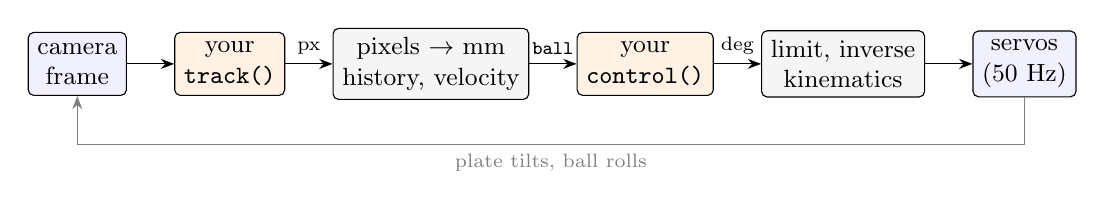
\begin{tikzpicture}[>=Stealth, box/.style={draw, rounded corners=2pt, minimum height=8mm, align=center, font=\small},
  node distance=6mm]
  \node[box, fill=blue!6] (cam) {camera\\frame};
  \node[box, right=of cam, fill=orange!10] (track) {your\\\texttt{track()}};
  \node[box, right=of track, fill=gray!8] (lib) {pixels $\to$ mm\\history, velocity};
  \node[box, right=of lib, fill=orange!10] (ctrl) {your\\\texttt{control()}};
  \node[box, right=of ctrl, fill=gray!8] (ik) {limit, inverse\\kinematics};
  \node[box, right=of ik, fill=blue!6] (servo) {servos\\(50 Hz)};
  \draw[->] (cam) -- (track);
  \draw[->] (track) -- node[above, font=\scriptsize]{px} (lib);
  \draw[->] (lib) -- node[above, font=\scriptsize]{\texttt{ball}} (ctrl);
  \draw[->] (ctrl) -- node[above, font=\scriptsize]{deg} (ik);
  \draw[->] (ik) -- (servo);
  \draw[->, gray] (servo.south) -- ++(0,-0.6) -| node[pos=0.25, below, font=\scriptsize]{plate tilts, ball rolls} (cam.south);
\end{tikzpicture}
\caption{One pass of the loop. Orange boxes are your code; grey boxes are the library.}
\label{fig:loop}
\end{figure}

%======================================================================
\section{Coordinates and sign conventions}\label{sec:coords}
%======================================================================
\begin{itemize}
  \item \textbf{Positions} are in millimetres on the plate surface. The origin is at the centre
        of the plate, and $x$ and $y$ are the plate's axes (\cref{fig:plate}). The plate has a
        radius of $100\un{mm}$; a $20\un{mm}$ ball falls off once its centre is beyond
        $100\un{mm}$.
  \item \textbf{Angles} are in degrees. \texttt{platform.angleX} is the angle the plate surface
        makes with the horizontal along $x$. A \emph{positive} value lifts the $+x$ edge, so the
        ball rolls towards $-x$. The same holds for \texttt{angleY}.
  \item \textbf{Time} is in seconds.
\end{itemize}

\begin{figure}[h]
\centering
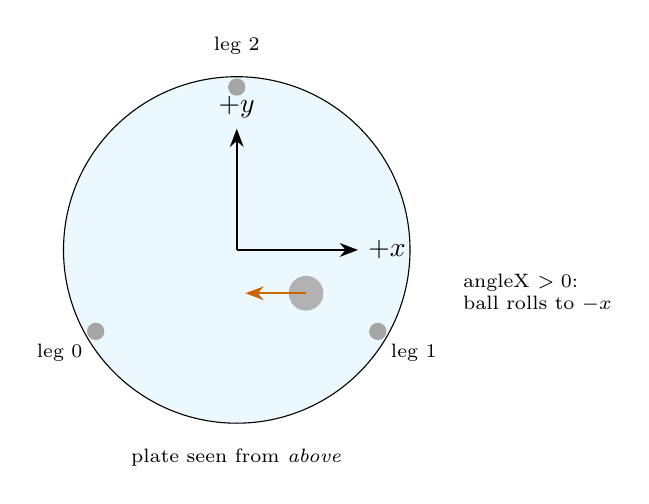
\begin{tikzpicture}[scale=0.022,>=Stealth]
  \draw[fill=cyan!8] (0,0) circle (100);
  \foreach \a/\n in {-150/0,-30/1,90/2} {
    \fill[gray!70] (\a:94) circle (5);
    \node[font=\scriptsize] at (\a:118) {leg \n};
  }
  \draw[->, thick] (0,0) -- (70,0) node[right] {$+x$};
  \draw[->, thick] (0,0) -- (0,70) node[above] {$+y$};
  \fill[gray!60] (40,-25) circle (10);
  \draw[->, orange!80!black, thick] (40,-25) -- (5,-25);
  \node[font=\scriptsize, align=left, anchor=west] at (125,-25) {angleX $>0$:\\ball rolls to $-x$};
  \node[font=\scriptsize] at (0,-120) {plate seen from \emph{above}};
\end{tikzpicture}
\caption{Plate coordinates seen from above. Leg 2 is on the $+y$ side.}
\label{fig:plate}
\end{figure}

%======================================================================
\section{What you get: the \texttt{Ball}}
%======================================================================
\begin{center}
\begin{tabularx}{\textwidth}{>{\ttfamily}lX}
\toprule
ball.found & \texttt{false} when \texttt{track()} did not find the ball this frame. The other
             fields then still hold the last good values.\\
ball.x, ball.y & Latest measured position [mm].\\
ball.vx, ball.vy & Filtered velocity [mm/s], see \cref{sec:velocity}.\\
ball.dt & Time since the previous \texttt{control()} call [s], normally $1/\text{fps}$.\\
ball.time & Current time [s].\\
ball.history(k) & The $k$-th previous measurement, with \texttt{.x}, \texttt{.y}, \texttt{.t}.
                  $k=0$ is the newest; up to 64 are kept.\\
ball.historySize() & How many samples are stored.\\
\bottomrule
\end{tabularx}
\end{center}

\subsection{How the position is measured}
Your tracker returns pixels. The library traces that pixel back out of the camera (undoing the
lens distortion), through the transparent plate (accounting for refraction), to the height of
the ball's centre. Two consequences:
\begin{itemize}
  \item The library uses the plate angle you \emph{commanded}, not the actual angle, because the
        firmware cannot know the actual angle. While the plate is still moving, this adds a small
        error.
  \item The measurement has noise from the camera image, a small systematic offset from
        perspective (about $1\un{mm}$ near the plate edge), and any artificial position noise you
        set.
\end{itemize}

\subsection{Velocity}\label{sec:velocity}
The velocity is estimated from consecutive positions and smoothed with a first-order
(exponential) filter:
\begin{equation}
  v_k=\alpha\,v_{k-1}+(1-\alpha)\,\frac{x_k-x_{k-1}}{t_k-t_{k-1}},
\end{equation}
where $\alpha$ is the \emph{velocity filter} in Setup~\textgreater~Control (default $0.5$). A
raw difference ($\alpha=0$) amplifies measurement noise: an error of $0.3\un{mm}$ at $30\un{fps}$
becomes velocity noise of order $10\un{mm/s}$. Smoothing reduces the noise but adds lag, about
$\tau=-\Delta t/\ln\alpha$, which is $48\un{ms}$ for $\alpha=0.5$ at $30\un{fps}$. If you prefer to
build your own estimator, use \texttt{ball.history()}.

%======================================================================
\section{What you set: the \texttt{Platform}}
%======================================================================
Set \texttt{platform.angleX} and \texttt{platform.angleY} in degrees. Then:
\begin{enumerate}
  \item The library clamps them to $\pm$\emph{Max plate angle} (Setup, default $8^\circ$).
  \item It turns them into a plate orientation. The plate normal is
        $\bm n\propto(-\tan\theta_x,\,-\tan\theta_y,\,1)$, so the two angles are independent and
        the order you set them in does not matter. The plate height stays fixed.
  \item It solves the inverse kinematics for the three crank angles and sends them as servo
        pulses. The servos take a new pulse every $20\un{ms}$, then move at their limited
        speed.
\end{enumerate}
If you ask for something out of reach, the command is ignored and a warning is shown.

\paragraph{Target.} \texttt{target.x}, \texttt{target.y} [mm] is where the ball should go. It is
set in the Setup tab: a fixed point, or a circle, square or figure eight. You can also move it
live from the Simulation tab.

%======================================================================
\section{Helpers}
%======================================================================
\subsection{\texttt{PID}}
\begin{lstlisting}
PID pid(kp, ki, kd);              // create once, outside control()
float u = pid.update(error, ball.dt);
pid.setDerivativeFilter(0.03f);   // optional: low-pass the D term (seconds)
pid.setIntegralLimit(50.0f);      // optional: anti-windup
pid.setOutputLimit(8.0f);         // optional: clamp the output
pid.reset();                      // forget the integral and history
\end{lstlisting}
Create PID objects \emph{outside} the function, so they keep their state between calls. Each
\texttt{update(e, dt)} computes exactly:
\begin{align}
  I_k &= \operatorname{clamp}\!\left(I_{k-1}+e_k\,\Delta t,\ \pm I_{\max}\right),\\
  d_k &= \frac{e_k-e_{k-1}}{\Delta t}\quad(0\text{ on the first call}),\qquad
  D_k = D_{k-1}+\frac{\Delta t}{\tau_d+\Delta t}\,(d_k-D_{k-1}),\\
  u_k &= \operatorname{clamp}\!\left(k_p e_k+k_i I_k+k_d D_k,\ \pm u_{\max}\right),
\end{align}
where $D_k=d_k$ when no derivative filter is set ($\tau_d=0$), and a limit of 0 means no limit.
The three terms of the last update are in \texttt{pid.lastP}, \texttt{lastI} and
\texttt{lastD}. Logging them is a good way to see which term is doing what.

\subsection{\texttt{log}, \texttt{clamp}, \texttt{printf}}
\texttt{log("name", value)} plots any value live in the Simulation tab, up to six series.
\texttt{clamp(v, lo, hi)} limits a value. \texttt{printf} prints to the output console; don't
call it every frame, because it is slow.

%======================================================================
\section{Timing and the Setup effects}\label{sec:timing}
%======================================================================
The ball sees your command later than you might think. Between the light leaving the ball and
the plate moving there are:
\begin{center}
\begin{tabular}{lll}
\toprule
Stage & Default & Setup control\\
\midrule
Exposure + rolling readout + transfer & $\approx24\un{ms}$ & Camera: exposure\\
Extra sensor delay & $0$ & Artificial effects: sensor delay\\
Your code on the FireBeetle & a few ms & measured $\times$ slowdown factor\\
Extra motor delay & $0$ & Artificial effects: motor delay\\
Waiting for the next servo pulse & $0$--$20\un{ms}$ & ---\\
Servo reaching the angle & $\sim30$--$100\un{ms}$ & --- (Simulated hardware: servos)\\
\bottomrule
\end{tabular}
\end{center}
The \emph{frame-rate cap} drops frames, so \texttt{control()} runs less often and
\texttt{ball.dt} grows. \emph{Position noise} adds random error to \texttt{ball.x} and
\texttt{ball.y}. These effects exist so you can see how each kind of non-ideality hurts a
controller, and how to design around it.

%======================================================================
\section{A model for design}\label{sec:model}
%======================================================================
For small angles, a ball rolling without slipping on a tilted plate accelerates at
\begin{equation}
  \ddot x=-\frac{g}{1+k}\,\sin\theta_x\approx-G\,\theta_x,\qquad
  G=\frac{g}{1+k}\cdot\frac{\pi}{180},
  \label{eq:plant}
\end{equation}
with $\theta_x$ in degrees. The factor $1+k$ is the rolling inertia: $k=\frac25$ for a solid ball,
about $\frac23$ for a thin-walled hollow ball \citep{bbpphysics}. Numerically:
\begin{center}
\begin{tabular}{lcc}
\toprule
Ball & $k$ & $G$ [mm/s$^2$ per degree]\\
\midrule
solid (steel, glass, plastic) & $2/5$ & $122$\\
hollow, thin wall & $\approx2/3$ & $103$\\
\bottomrule
\end{tabular}
\end{center}
The $x$ and $y$ axes are (almost) independent, so you can design one axis and copy it. In the
Laplace domain each axis is a double integrator with a delay $T$:
\begin{equation}
  \frac{X(s)}{\Theta(s)}=-\frac{G}{s^2}\,e^{-sT}.
\end{equation}
The full model also includes servo dynamics, friction and parasitic motion, and the simulator
uses all of it \citep{bbpphysics}. This simple model is what you design with.

\subsection{Why P alone does not work}
With $\theta_x=-k_pe$ and $e=x_t-x$ (a fixed target), \eqref{eq:plant} gives
$\ddot x+Gk_p\,x=Gk_p\,x_t$. That is an undamped oscillator: the ball swings through the target
forever. Any delay makes it grow. You need damping, which is the D term.

\subsection{PD design by pole placement}
With $\theta_x=-(k_pe+k_d\dot e)$ and $\dot e=-\dot x$:
\begin{equation}
  \ddot x+Gk_d\,\dot x+Gk_p\,x=Gk_p\,x_t
  \quad\Longrightarrow\quad
  \omega_n^2=Gk_p,\qquad2\zeta\omega_n=Gk_d.
\end{equation}
Choose the natural frequency $\omega_n$ (speed) and the damping $\zeta$ (overshoot), then
\begin{equation}
  k_p=\frac{\omega_n^2}{G},\qquad k_d=\frac{2\zeta\omega_n}{G}.
\end{equation}
\emph{Example.} With $\omega_n=3.45\un{rad/s}$ and $\zeta=0.85$, the gains are $k_p=0.097$ and
$k_d=0.048$, and the settling time is about $4/(\zeta\omega_n)\approx1.4\un{s}$. The starter code
uses $k_p=0.09$, $k_d=0.045$, which is this design rounded.

\subsection{The cost of delay}
A delay $T$ removes phase $\omega T$ at frequency $\omega$. Around the crossover frequency
$\omega_c\approx\omega_n$, the phase margin drops by
\begin{equation}
  \Delta\varphi\approx\omega_cT\ \text{rad}=57.3\,\omega_cT\ \text{degrees}.
\end{equation}
With the default $T\approx60\un{ms}$ and $\omega_c=3.5\un{rad/s}$, that is $12^\circ$. Add
$150\un{ms}$ of sensor delay and you lose another $30^\circ$, and the starter controller starts
to oscillate. A slower design (smaller $\omega_n$) tolerates more delay. This trade-off is the
central lesson of the Setup effects \citep{astrom2008feedback,franklin2015feedback}.

\subsection{The integral term and the dead zone}
Rolling resistance gives the ball a dead zone. On a plate tilted less than about
$\arctan c_{rr}$ (typically under $0.1^\circ$) it simply stays where it is. A PD controller then
leaves a small steady error. An integral term removes it, but integrates during large moves
too; limit it with \texttt{setIntegralLimit}. PID tuning in general is covered by
\citet{astrom1995pid}.

\subsection{Feedforward for moving targets}
To follow a moving target $x_t(t)$, the ball needs acceleration $\ddot x_t$. Adding the angle
that produces it, $\theta_{\mathrm{ff}}=-\ddot x_t/G$, lets the feedback handle only the errors.
For a circle of radius $R$ and period $P$, $\ddot x_t$ has magnitude $R(2\pi/P)^2$. That is
$25\un{mm/s^2}$, or $0.2^\circ$, for the default $40\un{mm}$, $8\un{s}$ circle.

%======================================================================
\section{The starter code}
%======================================================================
\begin{lstlisting}
#include <bbp/bbp.hpp>
using namespace bbp;

PID pidX(0.09f, 0.0f, 0.045f);
PID pidY(0.09f, 0.0f, 0.045f);

void control(const Ball& ball, const Target& target, Platform& platform) {
    if (!ball.found) {                  // lost the ball: level the plate
        platform.angleX = 0;
        platform.angleY = 0;
        return;
    }
    pidX.setDerivativeFilter(0.03f);
    pidY.setDerivativeFilter(0.03f);
    const float errorX = target.x - ball.x;
    const float errorY = target.y - ball.y;
    // ball too far to +x (error < 0) -> lift the +x edge (angle > 0)
    platform.angleX = -pidX.update(errorX, ball.dt);
    platform.angleY = -pidY.update(errorY, ball.dt);
    log("error x [mm]", errorX);
    log("error y [mm]", errorY);
}
\end{lstlisting}

\section{Things to try}
\begin{enumerate}
  \item Set $k_d=0$. Watch the ball oscillate, and explain why with the P-only analysis above.
  \item Add $100\un{ms}$, then $200\un{ms}$, of sensor delay. Re-tune with a smaller $\omega_n$.
  \item Replace the PID's derivative with \texttt{ball.vx}. How does the velocity filter change
        the result?
  \item Set the target to a circle. Add the feedforward term and compare the tracking error.
  \item Switch to a hollow ball (Simulated hardware). Which gain must change, and by how much?
\end{enumerate}

\bibliographystyle{plainnat}
\bibliography{references}

\end{document}
